\begin{frame}{Τρωτά σημεία μεθόδων ευθυγράμμισης}

  \begin{figure}
    \begin{frame}{Στόχος Σ2: Χρόνοι εκτέλεσης}

  \vspace{-3.5cm}
  \begin{figure}\centering
    \definecolor{c7}{RGB}{251,180,185}
\definecolor{c8}{RGB}{247,104,161}
\definecolor{c9}{RGB}{255,0,255}

% GNUPLOT: LaTeX picture with Postscript
\begingroup
  \makeatletter
  \providecommand\color[2][]{%
    \GenericError{(gnuplot) \space\space\space\@spaces}{%
      Package color not loaded in conjunction with
      terminal option `colourtext'%
    }{See the gnuplot documentation for explanation.%
    }{Either use 'blacktext' in gnuplot or load the package
      color.sty in LaTeX.}%
    \renewcommand\color[2][]{}%
  }%
  \providecommand\includegraphics[2][]{%
    \GenericError{(gnuplot) \space\space\space\@spaces}{%
      Package graphicx or graphics not loaded%
    }{See the gnuplot documentation for explanation.%
    }{The gnuplot epslatex terminal needs graphicx.sty or graphics.sty.}%
    \renewcommand\includegraphics[2][]{}%
  }%
  \providecommand\rotatebox[2]{#2}%
  \@ifundefined{ifGPcolor}{%
    \newif\ifGPcolor
    \GPcolorfalse
  }{}%
  \@ifundefined{ifGPblacktext}{%
    \newif\ifGPblacktext
    \GPblacktexttrue
  }{}%
  % define a \g@addto@macro without @ in the name:
  \let\gplgaddtomacro\g@addto@macro
  % define empty templates for all commands taking text:
  \gdef\gplfronttext{}%
  \gdef\gplfronttext{}%
  \makeatother
  \ifGPblacktext
    % no textcolor at all
    \def\colorrgb#1{}%
    \def\colorgray#1{}%
  \else
    % gray or color?
    \ifGPcolor
      \def\colorrgb#1{\color[rgb]{#1}}%
      \def\colorgray#1{\color[gray]{#1}}%
      \expandafter\def\csname LTw\endcsname{\color{white}}%
      \expandafter\def\csname LTb\endcsname{\color{black}}%
      \expandafter\def\csname LTa\endcsname{\color{black}}%
      \expandafter\def\csname LT0\endcsname{\color[rgb]{1,0,0}}%
      \expandafter\def\csname LT1\endcsname{\color[rgb]{0,1,0}}%
      \expandafter\def\csname LT2\endcsname{\color[rgb]{0,0,1}}%
      \expandafter\def\csname LT3\endcsname{\color[rgb]{1,0,1}}%
      \expandafter\def\csname LT4\endcsname{\color[rgb]{0,1,1}}%
      \expandafter\def\csname LT5\endcsname{\color[rgb]{1,1,0}}%
      \expandafter\def\csname LT6\endcsname{\color[rgb]{0,0,0}}%
      \expandafter\def\csname LT7\endcsname{\color[rgb]{1,0.3,0}}%
      \expandafter\def\csname LT8\endcsname{\color[rgb]{0.5,0.5,0.5}}%
    \else
      % gray
      \def\colorrgb#1{\color{black}}%
      \def\colorgray#1{\color[gray]{#1}}%
      \expandafter\def\csname LTw\endcsname{\color{white}}%
      \expandafter\def\csname LTb\endcsname{\color{black}}%
      \expandafter\def\csname LTa\endcsname{\color{black}}%
      \expandafter\def\csname LT0\endcsname{\color{black}}%
      \expandafter\def\csname LT1\endcsname{\color{black}}%
      \expandafter\def\csname LT2\endcsname{\color{black}}%
      \expandafter\def\csname LT3\endcsname{\color{black}}%
      \expandafter\def\csname LT4\endcsname{\color{black}}%
      \expandafter\def\csname LT5\endcsname{\color{black}}%
      \expandafter\def\csname LT6\endcsname{\color{black}}%
      \expandafter\def\csname LT7\endcsname{\color{black}}%
      \expandafter\def\csname LT8\endcsname{\color{black}}%
    \fi
  \fi
    \setlength{\unitlength}{0.0500bp}%
    \ifx\gptboxheight\undefined%
      \newlength{\gptboxheight}%
      \newlength{\gptboxwidth}%
      \newsavebox{\gptboxtext}%
    \fi%
    \setlength{\fboxrule}{0.5pt}%
    \setlength{\fboxsep}{1pt}%
\begin{picture}(8000.00,6000.00)%
    \gplgaddtomacro\gplfronttext{%
      \colorrgb{0.15,0.15,0.15}%
      \put(-52,4522){\makebox(0,0)[r]{\strut{}\small $100$}}%
      \colorrgb{0.15,0.15,0.15}%
      \put(-52,4940){\makebox(0,0)[r]{\strut{}\small $200$}}%
      \colorrgb{0.15,0.15,0.15}%
      \put(-52,5184){\makebox(0,0)[r]{\strut{}\small $300$}}%
      \colorrgb{0.15,0.15,0.15}%
      \put(-52,5358){\makebox(0,0)[r]{\strut{}\small $400$}}%
      \colorrgb{0.15,0.15,0.15}%
      \put(-52,5775){\makebox(0,0)[r]{\strut{}\small $800$}}%
      \colorrgb{0.15,0.15,0.15}%
      \put(-52,5910){\makebox(0,0)[r]{\strut{}\small $1000$}}%
      \colorrgb{0.15,0.15,0.15}%
      \put(468,4239){\makebox(0,0){\strut{}}}%
      \colorrgb{0.15,0.15,0.15}%
      \put(1244,4239){\makebox(0,0){\strut{}}}%
      \colorrgb{0.15,0.15,0.15}%
      \put(2020,4239){\makebox(0,0){\strut{}}}%
      \colorrgb{0.15,0.15,0.15}%
      \put(2795,4239){\makebox(0,0){\strut{}}}%
      \colorrgb{0.15,0.15,0.15}%
      \put(3571,4239){\makebox(0,0){\strut{}}}%
    }%
    \gplgaddtomacro\gplfronttext{%
      \colorrgb{0.00,0.00,0.00}%
      \put(3999,6159){\makebox(0,0){\strut{}Κατανομή αριθμού σαρώσεων χάρτη}}%
      \put(2019,6559){\makebox(0,0){\strut{}$\sigma_{\bm{M}} = 0.0$ m}}%
      \put(6019,6559){\makebox(0,0){\strut{}$\sigma_{\bm{M}} = 0.05$ m}}%
      \put(2999,6959){\makebox(0,0){\strut{}{\color{c7}{\rule[0.6mm]{0.5cm}{0.5mm}}}\small x1}}
      \put(3999,6959){\makebox(0,0){\strut{}{\color{c8}{\rule[0.6mm]{0.5cm}{0.5mm}}}\small uf}}
      \put(4999,6959){\makebox(0,0){\strut{}{\color{c9}{\rule[0.6mm]{0.5cm}{0.5mm}}}\small fm}}
    }%
    \gplgaddtomacro\gplfronttext{%
      \colorrgb{0.15,0.15,0.15}%
      \put(3908,4522){\makebox(0,0)[r]{\strut{}}}%
      \colorrgb{0.15,0.15,0.15}%
      \put(3908,4940){\makebox(0,0)[r]{\strut{}}}%
      \colorrgb{0.15,0.15,0.15}%
      \put(3908,5184){\makebox(0,0)[r]{\strut{}}}%
      \colorrgb{0.15,0.15,0.15}%
      \put(3908,5358){\makebox(0,0)[r]{\strut{}}}%
      \colorrgb{0.15,0.15,0.15}%
      \put(3908,5775){\makebox(0,0)[r]{\strut{}}}%
      \colorrgb{0.15,0.15,0.15}%
      \put(3908,5910){\makebox(0,0)[r]{\strut{}}}%
      \colorrgb{0.15,0.15,0.15}%
      \put(4428,4239){\makebox(0,0){\strut{}}}%
      \colorrgb{0.15,0.15,0.15}%
      \put(5204,4239){\makebox(0,0){\strut{}}}%
      \colorrgb{0.15,0.15,0.15}%
      \put(5980,4239){\makebox(0,0){\strut{}}}%
      \colorrgb{0.15,0.15,0.15}%
      \put(6755,4239){\makebox(0,0){\strut{}}}%
      \colorrgb{0.15,0.15,0.15}%
      \put(7531,4239){\makebox(0,0){\strut{}}}%
    }%
    \gplgaddtomacro\gplfronttext{%
    }%
    \gplgaddtomacro\gplfronttext{%
      \colorrgb{0.15,0.15,0.15}%
      \put(-52,2260){\makebox(0,0)[r]{\strut{}\small $0.0$}}%
      \colorrgb{0.15,0.15,0.15}%
      \put(-52,2683){\makebox(0,0)[r]{\strut{}\small $0.100$}}%
      \colorrgb{0.15,0.15,0.15}%
      \put(-52,3105){\makebox(0,0)[r]{\strut{}\small $0.200$}}%
      \colorrgb{0.15,0.15,0.15}%
      \put(-52,3528){\makebox(0,0)[r]{\strut{}\small $0.300$}}%
      \colorrgb{0.15,0.15,0.15}%
      \put(468,2040){\makebox(0,0){\strut{}}}%
      \colorrgb{0.15,0.15,0.15}%
      \put(1244,2040){\makebox(0,0){\strut{}}}%
      \colorrgb{0.15,0.15,0.15}%
      \put(2020,2040){\makebox(0,0){\strut{}}}%
      \colorrgb{0.15,0.15,0.15}%
      \put(2795,2040){\makebox(0,0){\strut{}}}%
      \colorrgb{0.15,0.15,0.15}%
      \put(3571,2040){\makebox(0,0){\strut{}}}%
    }%
    \gplgaddtomacro\gplfronttext{%
      \colorrgb{0.00,0.00,0.00}%
      \put(3999,3959){\makebox(0,0){\strut{}Κατανομή ολικού χρόνου εκτέλεσης [sec]}}%
    }%
    \gplgaddtomacro\gplfronttext{%
      \colorrgb{0.15,0.15,0.15}%
      \put(3908,2260){\makebox(0,0)[r]{\strut{}}}%
      \colorrgb{0.15,0.15,0.15}%
      \put(3908,2683){\makebox(0,0)[r]{\strut{}}}%
      \colorrgb{0.15,0.15,0.15}%
      \put(3908,3105){\makebox(0,0)[r]{\strut{}}}%
      \colorrgb{0.15,0.15,0.15}%
      \put(3908,3528){\makebox(0,0)[r]{\strut{}}}%
      \colorrgb{0.15,0.15,0.15}%
      \put(4428,2040){\makebox(0,0){\strut{}}}%
      \colorrgb{0.15,0.15,0.15}%
      \put(5204,2040){\makebox(0,0){\strut{}}}%
      \colorrgb{0.15,0.15,0.15}%
      \put(5980,2040){\makebox(0,0){\strut{}}}%
      \colorrgb{0.15,0.15,0.15}%
      \put(6755,2040){\makebox(0,0){\strut{}}}%
      \colorrgb{0.15,0.15,0.15}%
      \put(7531,2040){\makebox(0,0){\strut{}}}%
    }%
    \gplgaddtomacro\gplfronttext{%
    }%
    \gplgaddtomacro\gplfronttext{%
      \colorrgb{0.15,0.15,0.15}%
      \put(-52,60){\makebox(0,0)[r]{\strut{}\small $0.0$}}%
      \colorrgb{0.15,0.15,0.15}%
      \put(-52,483){\makebox(0,0)[r]{\strut{}\small $0.050$}}%
      \colorrgb{0.15,0.15,0.15}%
      \put(-52,905){\makebox(0,0)[r]{\strut{}\small $0.100$}}%
      \colorrgb{0.15,0.15,0.15}%
      \put(-52,1328){\makebox(0,0)[r]{\strut{}\small $0.150$}}%
      \colorrgb{0.15,0.15,0.15}%
      \put(468,-160){\makebox(0,0){\strut{}$0.01$}}%
      \colorrgb{0.15,0.15,0.15}%
      \put(1244,-160){\makebox(0,0){\strut{}$0.03$}}%
      \colorrgb{0.15,0.15,0.15}%
      \put(2020,-160){\makebox(0,0){\strut{}$0.05$}}%
      \colorrgb{0.15,0.15,0.15}%
      \put(2795,-160){\makebox(0,0){\strut{}$0.10$}}%
      \colorrgb{0.15,0.15,0.15}%
      \put(3571,-160){\makebox(0,0){\strut{}$0.20$}}%
    }%
    \gplgaddtomacro\gplfronttext{%
      \colorrgb{0.15,0.15,0.15}%
      \put(3999,-490){\makebox(0,0){\strut{}Τυπική απόκλιση διαταραχών $\sigma_R$ [m]}}%
      \colorrgb{0.00,0.00,0.00}%
      \put(3999,1759){\makebox(0,0){\strut{}Κατανομή ολικού χρόνου εκτέλεσης [sec] (Αναγωγή σε αναπαράσταση χάρτη μέσω πλέγματος)}}%
    }%
    \gplgaddtomacro\gplfronttext{%
      \colorrgb{0.15,0.15,0.15}%
      \put(3908,60){\makebox(0,0)[r]{\strut{}}}%
      \colorrgb{0.15,0.15,0.15}%
      \put(3908,483){\makebox(0,0)[r]{\strut{}}}%
      \colorrgb{0.15,0.15,0.15}%
      \put(3908,905){\makebox(0,0)[r]{\strut{}}}%
      \colorrgb{0.15,0.15,0.15}%
      \put(3908,1328){\makebox(0,0)[r]{\strut{}}}%
      \colorrgb{0.15,0.15,0.15}%
      \put(4428,-160){\makebox(0,0){\strut{}$0.01$}}%
      \colorrgb{0.15,0.15,0.15}%
      \put(5204,-160){\makebox(0,0){\strut{}$0.03$}}%
      \colorrgb{0.15,0.15,0.15}%
      \put(5980,-160){\makebox(0,0){\strut{}$0.05$}}%
      \colorrgb{0.15,0.15,0.15}%
      \put(6755,-160){\makebox(0,0){\strut{}$0.10$}}%
      \colorrgb{0.15,0.15,0.15}%
      \put(7531,-160){\makebox(0,0){\strut{}$0.20$}}%
    }%
    \gplgaddtomacro\gplfronttext{%
    }%
    \put(0,0){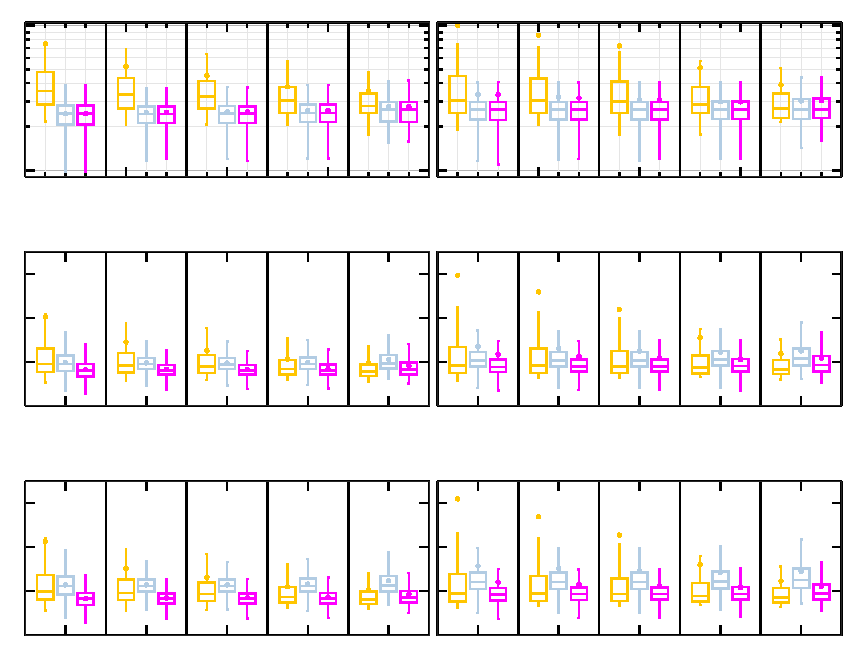
\includegraphics{./figures/parts/02/chapters/04/sections/05/boxplots_iterations}}%
    \gplfronttext
  \end{picture}%
\endgroup

  \end{figure}


  \placebottom
  \tiny [1] C. H. Walsh and S. Karaman, ``CDDT: Fast Approximate 2D Ray Casting for Accelerated Localization,", \textit{IEEE International Conference on Robotics and Automation}, 2018

\note{\footnotesize
Πάμε τώρα στο δεύτερο στόχο. Σε αυτή τη διαφάνεια βλέπουμε τους χρόνους
εκτέλεσης των τριών εκδόσεων του fsm2 για κάθε τιμή θορύβου μέτρησης και
διαφθοράς του χάρτη. Στην άνω σειρά βλέπουμε τα ευθεία αποτελέσματα από την
πειραματική διαδικασία και στην κάτω σειρά τους χρόνους εκτέλεσης που θα είχαν
οι μέθοδοι εάν ο χάρτης αναπαρίστατο ως εικόνα. Η διαφορά ανάμεσα στις δύο
αναπαραστάσεις είναι μεγάλη λόγω του χρόνου υπολογισμού εικονικών σαρώσεων που
είναι η πιό δαπανηρή πράξη, και που στην περίπτωση της αναπαράστασης μέσω
εικόνας μπορεί να γίνει στο ένα τρίτο του χρόνου σε σχέση με τον τρόπου που την
έχω υλοποιήσει εδώ. Τώρα: ο στόχος μας εδώ είναι κάθε μέθοδος να εκτελείται σε
μεγαλύτερη συχνότητα από τη συχνότητα παραγωγής εκτιμήσεων από το σύστημα που
εκτελεί το pose tracking, η οποία δεν έχει ακριβή ορισμό.  Στην πράξη αυτό που
θα θέλαμε είναι η συχνότητα εκτέλεσης να είναι τουλάχιστον 5 Hz.
Ο χαμηλότερος ρυθμός εκτέλεσης είναι της μεθόδου x1 όταν ο χάρτης είναι
διεφθαρμένος, κατά μέσο όρο στα 6.5 Hz, ενώ οι υπόλοιπες δύο μέθοδοι λειτουργούν
με τιμή περίπου στα 13 με 20 Hz.}

\end{frame}

  \end{figure}

\note{\footnotesize
Και εδώ φτάνουμε στο δεύτερο τρωτό σημείο, το οποίο αφορά σε όλες τις μεθόδους
ευθυγράμμισης της βιβλιογραφίας, επειδή ακριβώς όλες χρησιμοποιούν αυτόν το
μηχανισμό: το οποίο είναι το πρόβλημα του θορύβου μέτρησης.}
\end{frame}
